\chapter{操作系统的输入/输入系统}\label{cha:latex-brief-intro}

\section{实验内容}
实现简单的 I/O,从键盘输入字符的中断开始;获取并打印扫描码;创建对应打印扫描码解析数组,打印对应字符。
\section{代码分析}

\subsection{核心数据结构}

\begin{table}[H]
\begin{center}
\caption{keyboard.h缓冲区KB$\_$INPUT}
\begin{tabular}{|c|l|l|}
\hline
\multirow{4}{*}{缓冲区 KB\_INPUT} & p\_head                & 指向缓冲区中下一个空闲位置 \\ \cline{2-3} 
                               & p\_tail                & 指向键盘任务应处理的字节  \\ \cline{2-3} 
                               & Count                  & 缓冲区中字节数       \\ \cline{2-3} 
                               & buf{[}KB\_IN\_BYTES{]} & 缓冲区           \\ \hline
\end{tabular}
\end{center}
\end{table}


\subsection{关键代码分析}
\begin{enumerate}

    \item 键盘中断处理程序:
    \begin{lstlisting}[language=C]
    PUBLIC void keyboard_handler(int irq)
    {
        disp_str("str");
    }
    \end{lstlisting}
    
    \item 打开键盘中断:
    \begin{lstlisting}[language=C]
    PUBLIC void init_keyboard()
    {
        put_irq_handler(KEYBOARD_IRQ, keyboard_handler); /* 设定键盘中断处理程序 */
        enable_irq(KEYBOARD_IRQ); /* 开启键盘中断 */
    }
    \end{lstlisting}
    
    \item 调用 \texttt{init\_keyboard}:
    \begin{lstlisting}[language=C]
    PUBLIC int kernel_main()
    {
        // ...
        init_keyboard();
        // ...
    }
    \end{lstlisting}
    
    \item 修改后的键盘中断:
    \begin{lstlisting}[language=C]
    PUBLIC void keyboard_handler(int irq)
    {
        /* disp_str("*"); */
        u8 scan_code = in_byte(0x60);
        disp_int(scan_code);
    }
    \end{lstlisting}
    
    \item 扫描码解析数组:
    \begin{lstlisting}[language=C]
    u32 keymap[NR_SCAN_CODES * MAP_COLS] = {
        /* 0x00 - none */ 0, 0, 0,
        /* 0x01 - ESC */ ESC, ESC, 0,
        /* 0x02 - '1' */ '1', '!', 0,
        // ...
    };
    \end{lstlisting}
    
    \item 键盘缓冲区:
    \begin{lstlisting}[language=C]
    typedef struct s_kb {
        char* p_head;   /* 指向缓冲区中下一个空闲位置 */
        char* p_tail;   /* 指向键盘任务应处理的字节 */
        int count;      /* 缓冲区中共有多少字节 */
        char buf[KB_IN_BYTES]; /* 缓冲区 */
    } KB_INPUT;
    \end{lstlisting}
    
    \item 修改后的 \texttt{keyboard\_handler}:
    \begin{lstlisting}[language=C]
    PRIVATE KB_INPUT kb_in;
    
    /* keyboard_handler */
    PUBLIC void keyboard_handler(int irq)
    {
        u8 scan_code = in_byte(KB_DATA);
        if (kb_in.count < KB_IN_BYTES) {
            *(kb_in.p_head) = scan_code;
            kb_in.p_head++;
            if (kb_in.p_head == kb_in.buf + KB_IN_BYTES) {
                kb_in.p_head = kb_in.buf;
            }
            kb_in.count++;
        }
    }
    \end{lstlisting}
    
    \item 修改后的 \texttt{init\_keyboard}:
    \begin{lstlisting}[language=C]
    PUBLIC void init_keyboard()
    {
        kb_in.count = 0;
        kb_in.p_head = kb_in.p_tail = kb_in.buf;
        put_irq_handler(KEYBOARD_IRQ, keyboard_handler); /* 设定键盘中断处理程序 */
        enable_irq(KEYBOARD_IRQ); /* 开键盘中断 */
    }
    \end{lstlisting}
    
    \item 时钟中断处理函数 \texttt{init\_clock}:
    \begin{lstlisting}[language=C]
    PUBLIC void init_clock()
    {
        /* 初始化 8253 PIT */
        out_byte(TIMER_MODE, RATE_GENERATOR);
        out_byte(TIMER0, (u8) (TIMER_FREQ/HZ));
        out_byte(TIMER0, (u8) ((TIMER_FREQ/HZ) >> 8));
        put_irq_handler(CLOCK_IRQ, clock_handler); /* 设定时钟中断处理程序 */
        enable_irq(CLOCK_IRQ); /* 让 8259A 可以接收时钟中断 */
    }
    \end{lstlisting}
    
    \item 键盘读取的 \texttt{tty} 任务:
    \begin{lstlisting}[language=C]
    PUBLIC void task_tty()
    {
        while (1) {
            keyboard_read();
        }
    }
    \end{lstlisting}
    
    \item 键盘读取函数 \texttt{keyboard\_read()}:
    \begin{lstlisting}[language=C]
    PUBLIC void keyboard_read()
    {
        u8 scan_code;
        if (kb_in.count > 0) {
            disable_int();
            scan_code = *(kb_in.p_tail);
            kb_in.p_tail++;
            if (kb_in.p_tail == kb_in.buf + KB_IN_BYTES) {
                kb_in.p_tail = kb_in.buf;
            }
            kb_in.count--;
            enable_int();
            disp_int(scan_code);
        }
    }
    \end{lstlisting}
    
    \item \texttt{disable\_int} 与 \texttt{enable\_int}:
    \begin{lstlisting}[language=C]
    /* void disable_int(); */
    /* disable_int: */
    /* cli */
    /* ret */
    
    /* void enable_int(); */
    /* enable_int: */
    /* sti */
    /* ret */
    \end{lstlisting}
    
    \item 解析扫描码:
    \begin{lstlisting}[language=C]
    PUBLIC void keyboard_read()
    {
        u8 scan_code;
        char output[2];
        int make; /* TRUE: make; FALSE: break. */
    
        memset(output, 0, 2);
        if (kb_in.count > 0) {
            disable_int();
            scan_code = *(kb_in.p_tail);
            kb_in.p_tail++;
            if (kb_in.p_tail == kb_in.buf + KB_IN_BYTES) {
                kb_in.p_tail = kb_in.buf;
            }
            kb_in.count--;
            enable_int();
            /* 下面开始解析扫描码 */
            if (scan_code == 0xE1) {
                /* 暂时不做任何操作 */
            }
            else if (scan_code == 0xE0) {
                /* 暂时不做任何操作 */
            }
            else {
                /* 下面处理可打印字符 */
                /* 首先判断 Make Code 还是 Break Code */
                make = (scan_code & FLAG_BREAK ? FALSE : TRUE);
                /* 如果是 Make Code 就打印,是 Break Code 则不做处理 */
                if (make) {
                    output[0] = keymap[(scan_code & 0x7F) * MAP_COLS];
                    disp_str(output);
                }
            }
        }
    }
    \end{lstlisting}
\end{enumerate}


\section{调试过程及结果分析}
使用make指令编译,bochs指令运行,可以看到,当我们敲击键盘之后,程序中出现了一个“*”的字符,但当我们再次敲击键盘后,键盘却不会再次相应,即屏幕上不会出现第二个“*”字符,而且在terminal中可以看到栈溢出的报错信息。结果如下图8-1所示:
\begin{figure}[H]
  \centering
  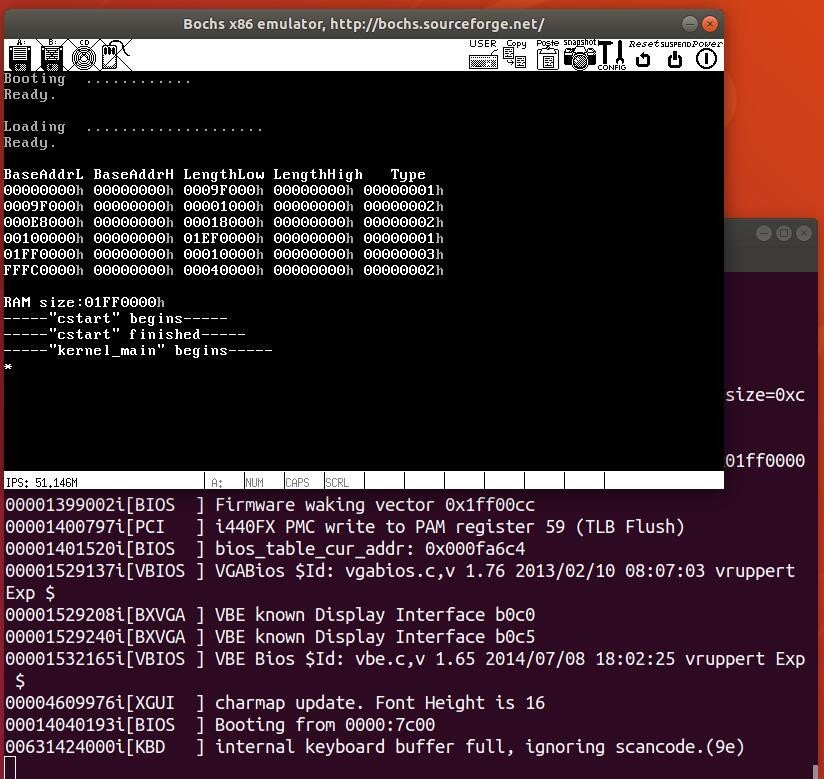
\includegraphics[width=0.8\textwidth]{figures/chapter8/8-1.jpg}
  \caption{键盘中断处理程序打印星号}
  \label{fig:1}
\end{figure}

在此处,我们调用键盘中断,在敲击键盘后出现了一个“*”字符,代表我们的键盘中断是准确无误的,但它目前只能相应一次键盘敲击。结合栈溢出的报错信息,我们可以每次输出缓冲区中字符对应的解析码。运行结果如下图8-2所示:
\begin{figure}[H]
  \centering
  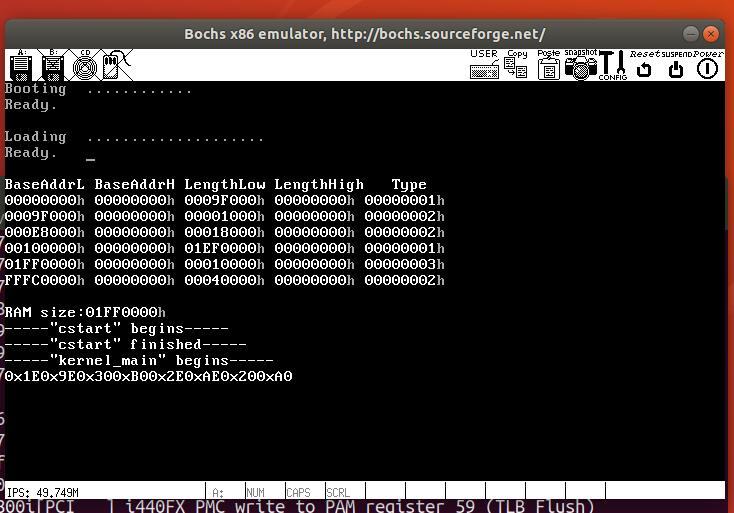
\includegraphics[width=0.8\textwidth]{figures/chapter8/8-2.jpg}
  \caption{读取缓冲区并打印解析码}
  \label{fig:2}
\end{figure}

在上图所示调试过程中,我们连续连续敲击了四个键:字符“a”、字符“b”、字符“c”和字符“d”,而实验结果则一共出现了 8 组数字,分别对应于字符“a”、“b”、“c”和“d”的 Make Code 和 Break Code。可以看到,我们目前的程序已经不会再卡死,而是可以相应多次键盘敲击过程,并且打印出扫描码。对于这一点,则涉及到键盘控制器 8042 芯片和键盘编码器 8048 芯片,它们会监视键盘的输入,并把适当的数据传给计算机。而对于敲击键盘的动作,则会产生扫描码,分别为按下一个按键或保持一个按键的 Make Code 和键盘弹起时的 Break Code,这些扫描码可以通过 in al,60h 读取,并且只有我们将扫描码从缓冲区中读出来后,8042 才能继续响应新的按键,这也解释了我们在之前的实验中只打印一个“*”的原因。接下来我们通过扫描码解析数组 keymap[ ],建立字符与解析码之间的映射关系,再次调试结果如下图8-3所示:
\begin{figure}[H]
  \centering
  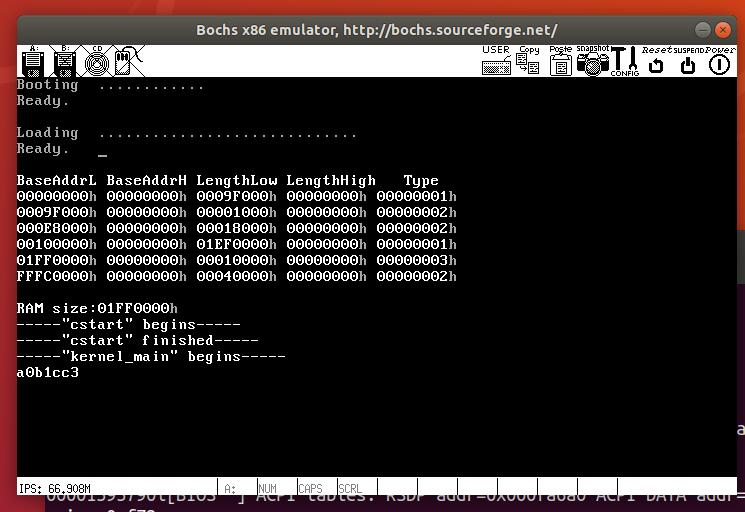
\includegraphics[width=0.8\textwidth]{figures/chapter8/8-3.jpg}
  \caption{输出正确的小写字符和数字}
  \label{fig:3}
\end{figure}

可以看到,目前我们的程序已经可以对小写 a-z 以及 0-9 产生正常响应,但仍然无法打印出大写字母,对 shift、alt、ctrl等按键则会输出意义不明的字符。由于我们已经知晓键盘敲击产生字符的原理,根据组合键的Make Code和Break Code专门处理,这一点不难实现。实现后运行结果如下图8-4所示:
\begin{figure}[H]
  \centering
  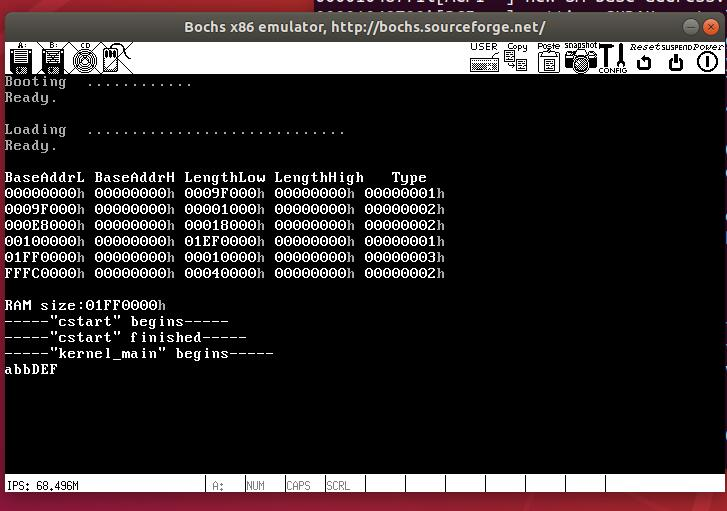
\includegraphics[width=0.8\textwidth]{figures/chapter8/8-4.jpg}
  \caption{输出组合键}
  \label{fig:4}
\end{figure}

\section{实验总结}

本次实验研究的是输入与输出。经过这次实验,我对电脑如何将外界输入处理成对应显示有了更深的了解。一次按键对应一个输出字符很好理解,但对于各种复杂组合键的实现方法,了解到敲击键盘按下和松开分别会有两个扫描码后,这才从原理上完全理解。\par
总而言之,第七个实验的任务是实现操作系统的输入输出系统。最初的时候,我们的键盘只能输入一个星号,因为这个程序并没有从缓冲区读取扫描码,相应的芯片不能及时响应按键。然后我们添加 in$\_$byte(0x60)指令,这样就可以多次输入了。接着,我们再次修改代码,使得屏幕能够显示按键的扫描码 MakeCode 和 BreakCode。接下来,我们引入扫描码解析数组,再使用键盘缓冲区存放暂未处理的输入。我们首先忽略 0xE0 和 0xE1。这样所有的小写字母就可以正常输出了。然后增加处理 Shift 的代码,这样就能够识别大写字母和特殊字符了。整理的实验七实验思维导图如下图 8-5 所示:
\begin{figure}[H]
  \centering
  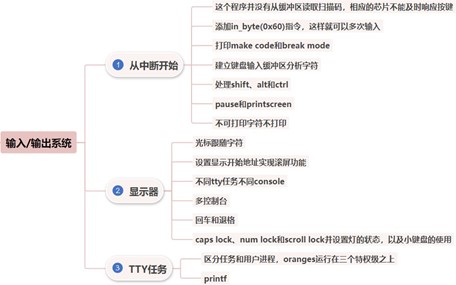
\includegraphics[width=0.8\textwidth]{figures/chapter8/8-5.jpg}
  \caption{实验七思维导图}
  \label{fig:5}
\end{figure}
